\RequirePackage{scrlfile}
\PreventPackageFromLoading{subfig}
\documentclass[10pt]{beamer}


\usetheme[
outer/progressbar=frametitle,
outer/numbering=none
]{metropolis}

\definecolor{light-gray}{gray}{0.7}


\pgfdeclareimage[width=\paperwidth]{mybackground}{melbourne.jpg}

%\usepackage{MnSymbol,wasysym}
\usepackage{subcaption,color,colortbl}
\usepackage{svg}
\usepackage{hyperref}
\usepackage{amsmath}
\usepackage{graphicx}
\usepackage{animate}

\usepackage{array}

\newcolumntype{M}[1]{>{\centering\arraybackslash}m{#1}}
\newcolumntype{N}{@{}m{0pt}@{}}

\usepackage[absolute,overlay]{textpos}

\usepackage{fontspec}
\setmainfont % load font from path
[
	Path = /usr/share/fonts/opentype/fira/,
	Extension = .otf,
	UprightFont = FiraSans-Regular,
	BoldFont = FiraSans-SemiBold,
]
{helvetica}
%\setmainfont[Ligatures=TeX]{helvetica-regular.otf}
\let\sfdefault\rmdefault

\definecolor{gray}{HTML}{333333}
\definecolor{teal}{HTML}{3CBCBC}
\definecolor{maroon}{HTML}{800000}
\definecolor{dteal}{HTML}{005566}
\definecolor{dgreen}{HTML}{003300}
\definecolor{dblue}{HTML}{000033}
\definecolor{dred}{HTML}{330000}
\setbeamercolor{frametitle}{bg=gray}
\setbeamercolor{alerted text}{fg=teal}

\usepackage{appendixnumberbeamer}


\usepackage{booktabs}
\usepackage{tikz}

\usepackage{pgfplots}
\usepgfplotslibrary{dateplot}

\usepackage{xspace}
\newcommand{\themename}{\textbf{\textsc{metropolis}}\xspace}



\usebackgroundtemplate%
{%
	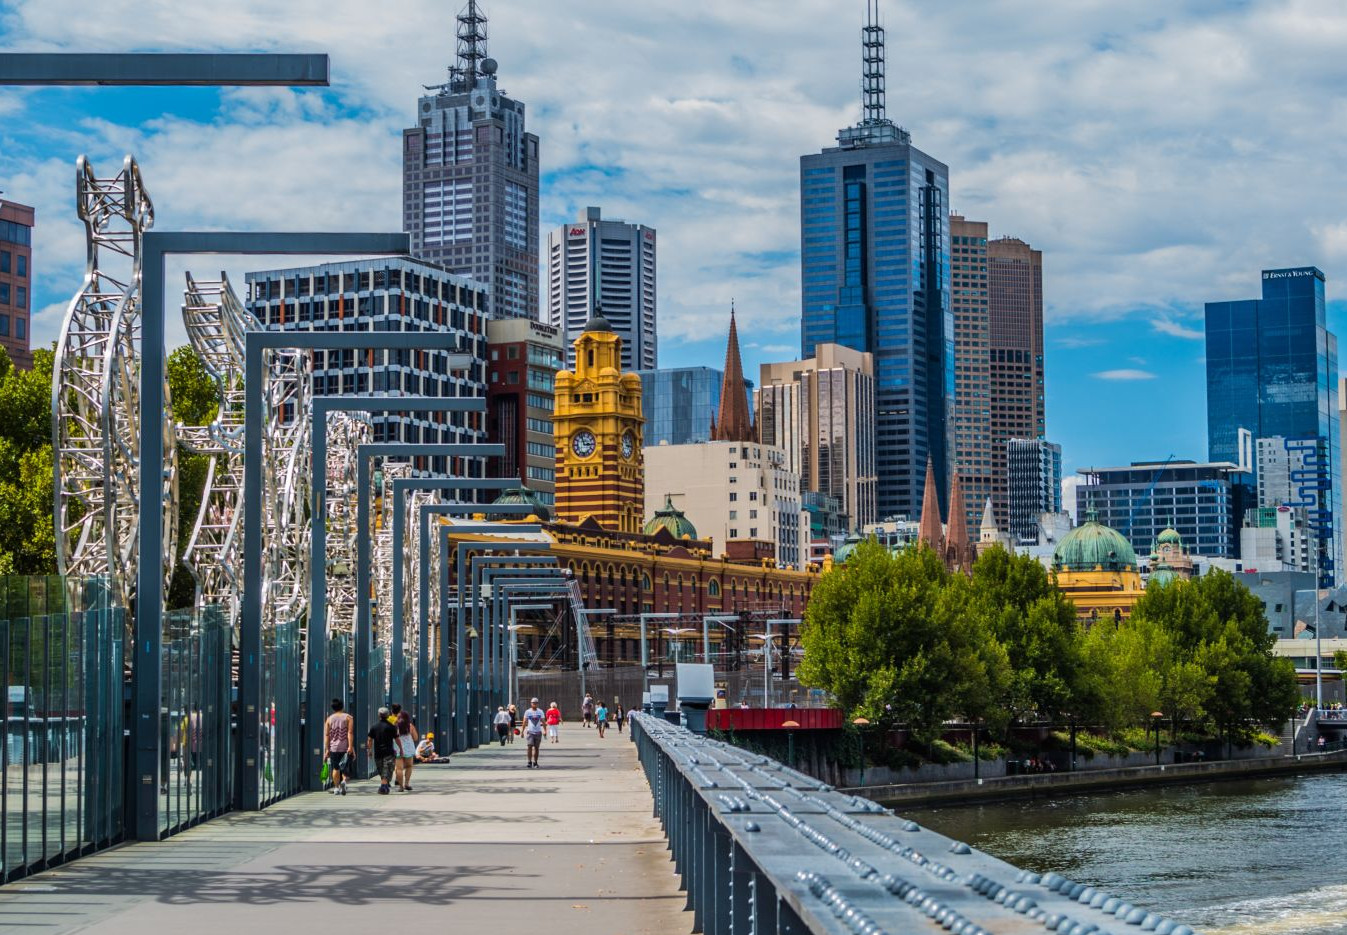
\includegraphics[width=\paperwidth,height=\paperheight]{figures/melbourne.jpg}%

}

\title{\LARGE Location Privacy \& Security Workshop}
\subtitle{\small At the 10th International Conference on Geographic Information Science}
\date{}
\author{}
\institute{}
\titlegraphic{
	\vspace{5.5cm}	
	\hspace*{7.3cm}

	%\put(1,120){\colorbox{gray!20}{\framebox(10,3){.}}}
}



% \titlegraphic{\hfill\includegraphics[height=1.5cm]{logo.pdf}}

\begin{document}

	\begin{frame}
		
			\begin{tikzpicture}[overlay]
			\draw [transform canvas={yshift=-7.7cm,xshift=-1.1cm}, draw=white, fill=white, opacity=0.8] (0,0) rectangle (13.1,5.9);
			\end{tikzpicture}
			\titlepage
	\end{frame}

%	\begin{frame}{Table of contents}
%		\setbeamertemplate{section in toc}[sections numbered]
%		\tableofcontents[hideallsubsections]
%	\end{frame}
	
	%\section{Introduction}

\usebackgroundtemplate%
{
}

	\begin{frame}{Why LoPaS 2018?}
		\Large What was the motivation for this workshop?
	\end{frame}

	\begin{frame}{LoPaS '18}
		\begin{figure}[H]
			\vspace{4mm}
			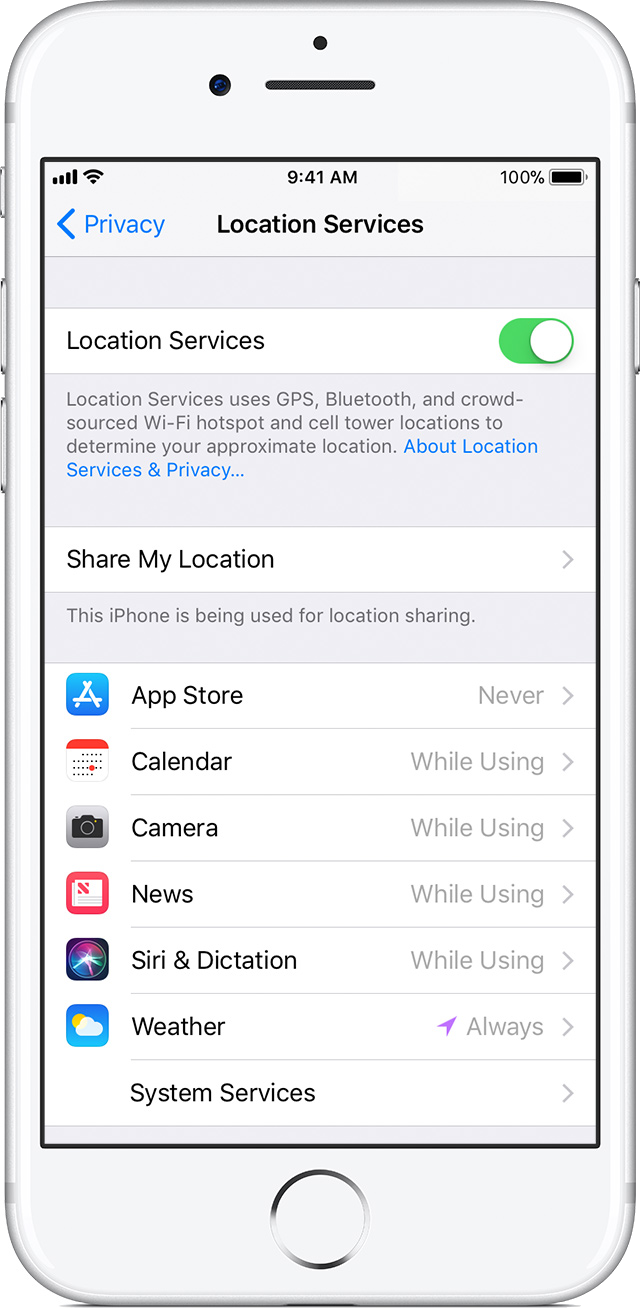
\includegraphics[width=0.72\textwidth]{figures/locationprivacy.png}
		\end{figure}
	\end{frame}

	\begin{frame}{LoPaS '18}
		\begin{minipage}[c]{0.65\textwidth}
			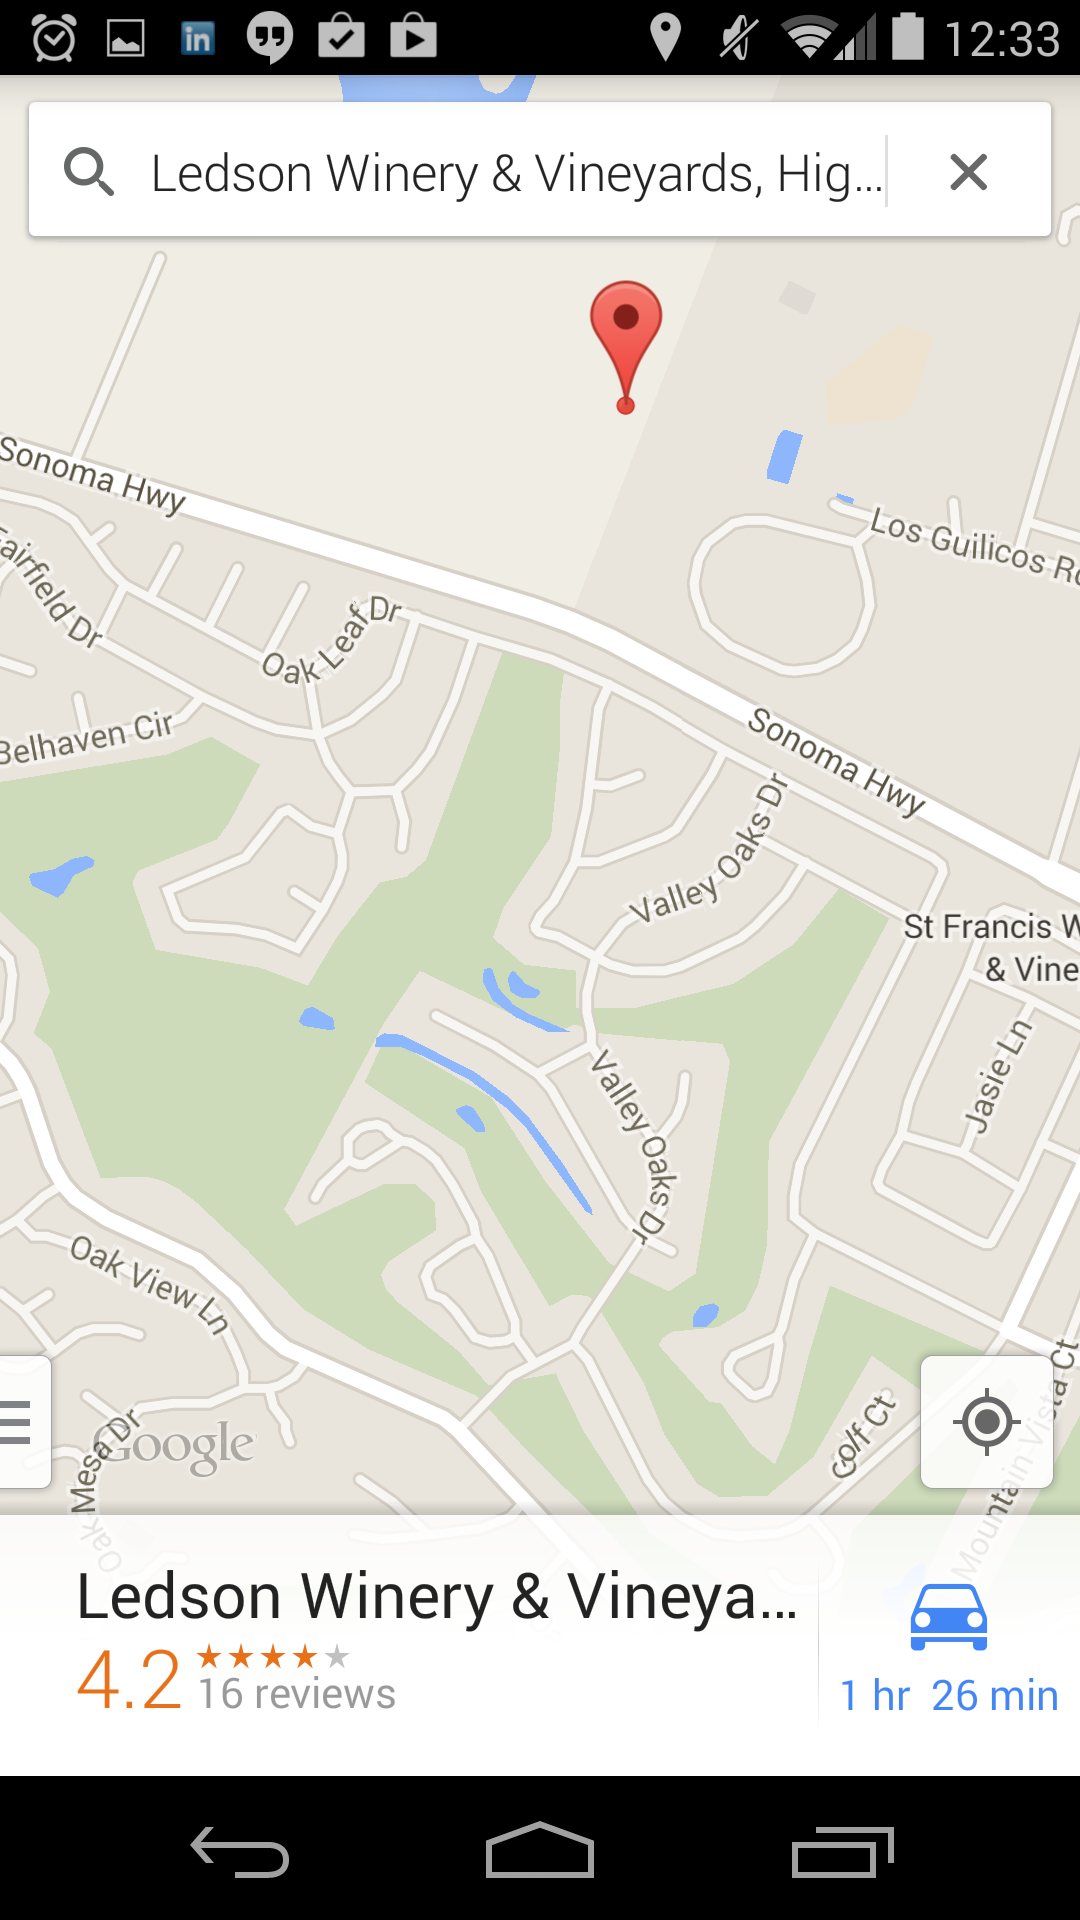
\includegraphics[width=0.49\textwidth]{figures/screen1.jpg}
			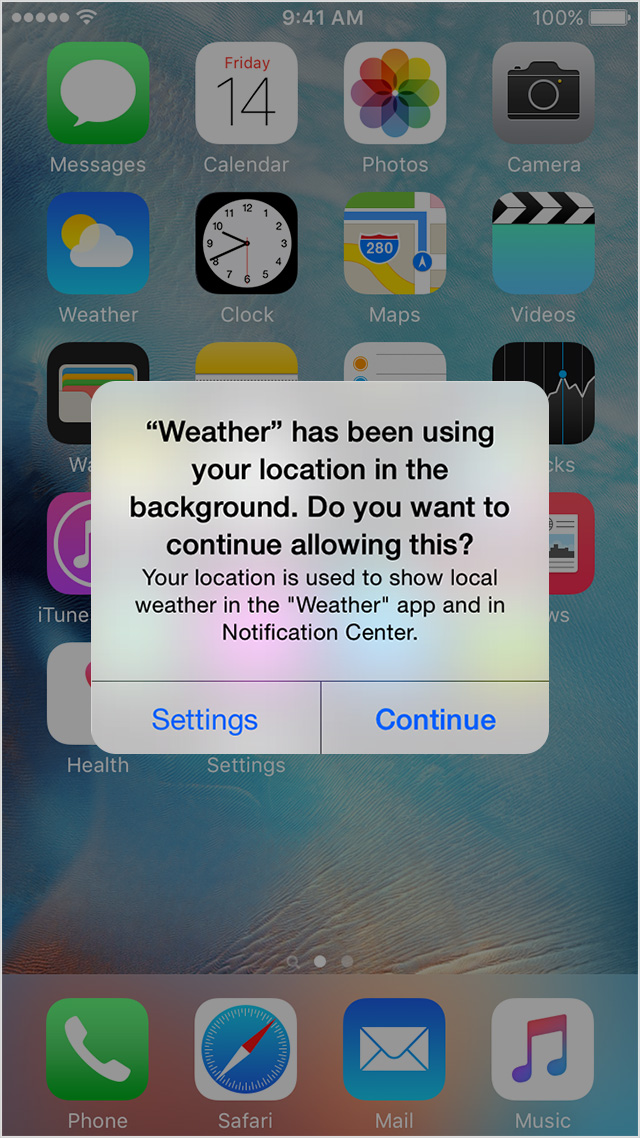
\includegraphics[width=0.49\textwidth]{figures/screen2.jpg}
		\end{minipage}
		\hfill
		\begin{minipage}[c]{0.34\textwidth}
			
\includegraphics[width=\textwidth]{figures/sm.jpg}
			
			\vspace{5mm}
			
			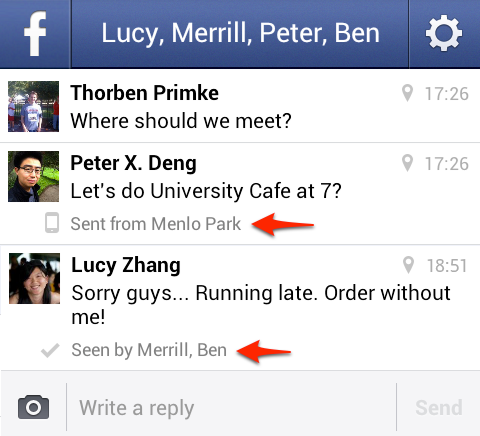
\includegraphics[width=\textwidth]{figures/screen3.jpg}
		\end{minipage}
	\end{frame}

	\begin{frame}{How is Location Privacy \& Security Understood?}
			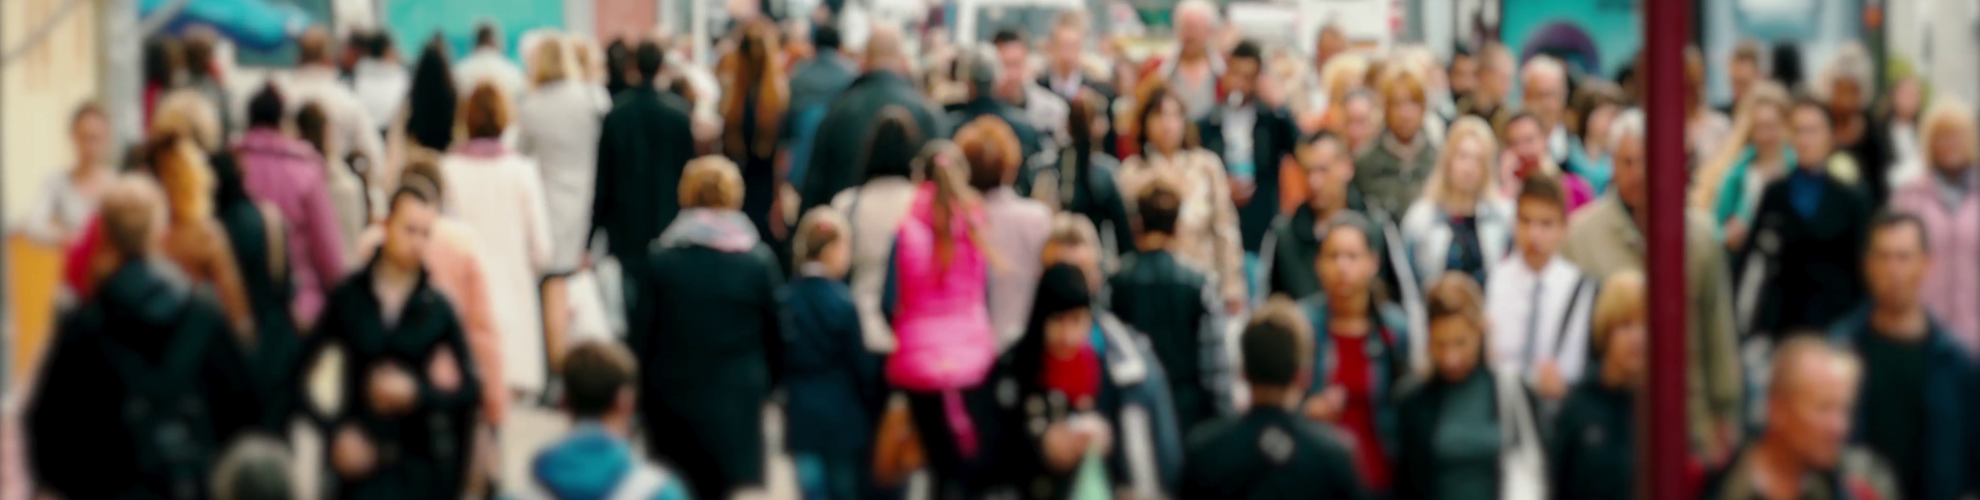
\includegraphics[width=\textwidth]{figures/people.png}
			\pause
			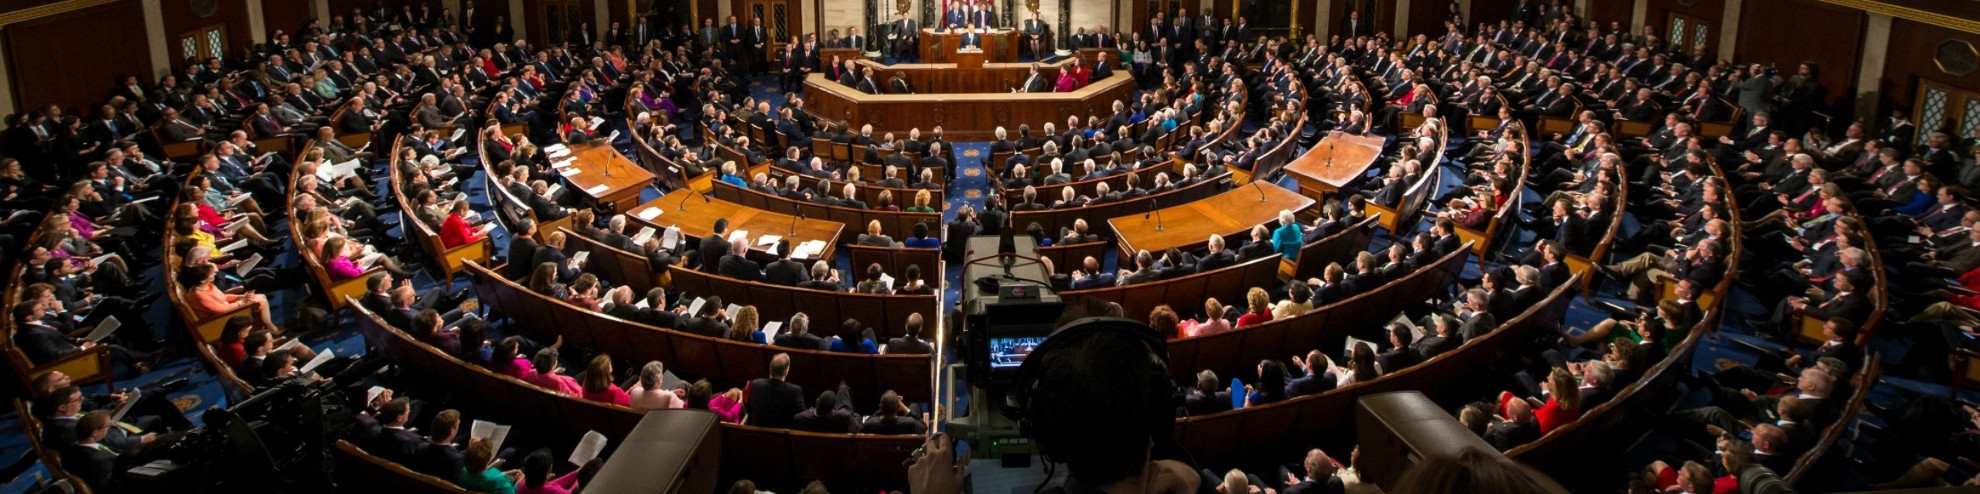
\includegraphics[width=\textwidth]{figures/congress.jpg}
			\pause
			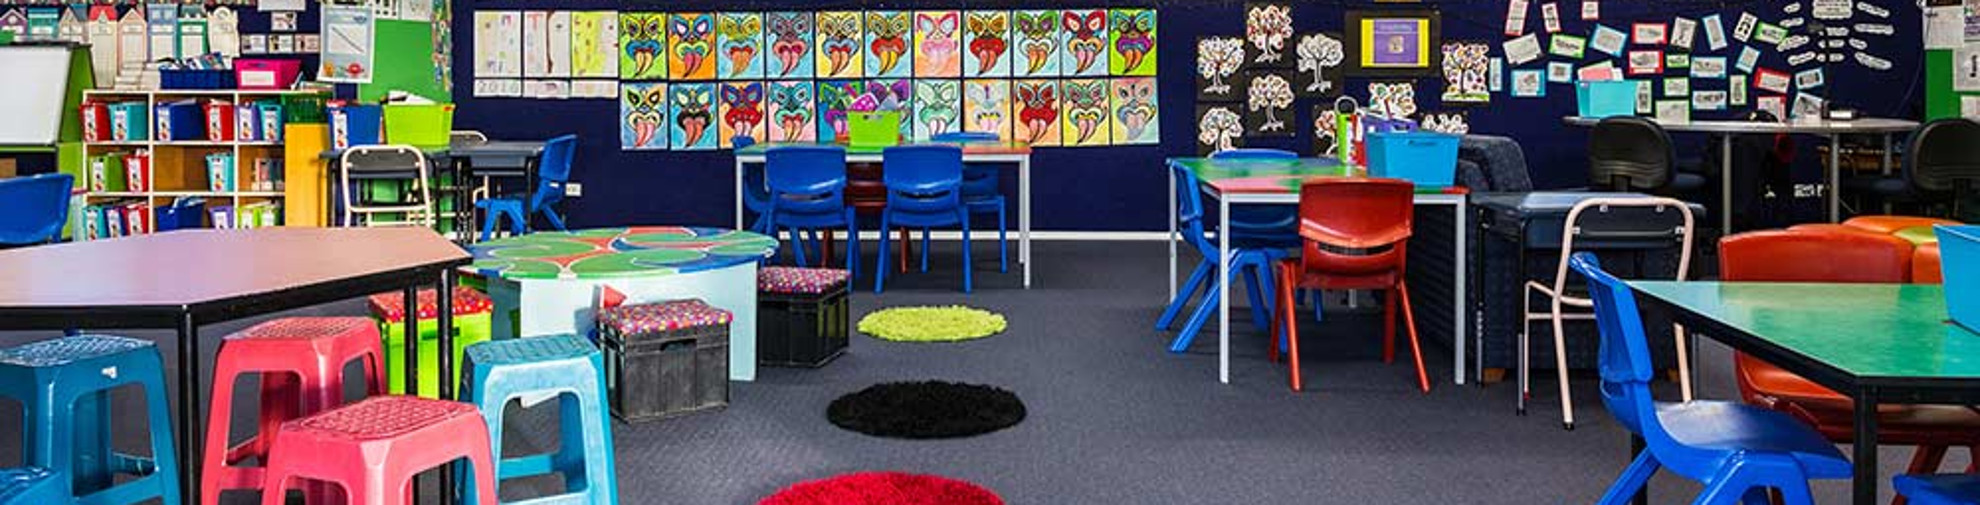
\includegraphics[width=\textwidth]{figures/kids.jpg}
	\end{frame}

	\begin{frame}{How is Location Privacy \& Security Understood?}
		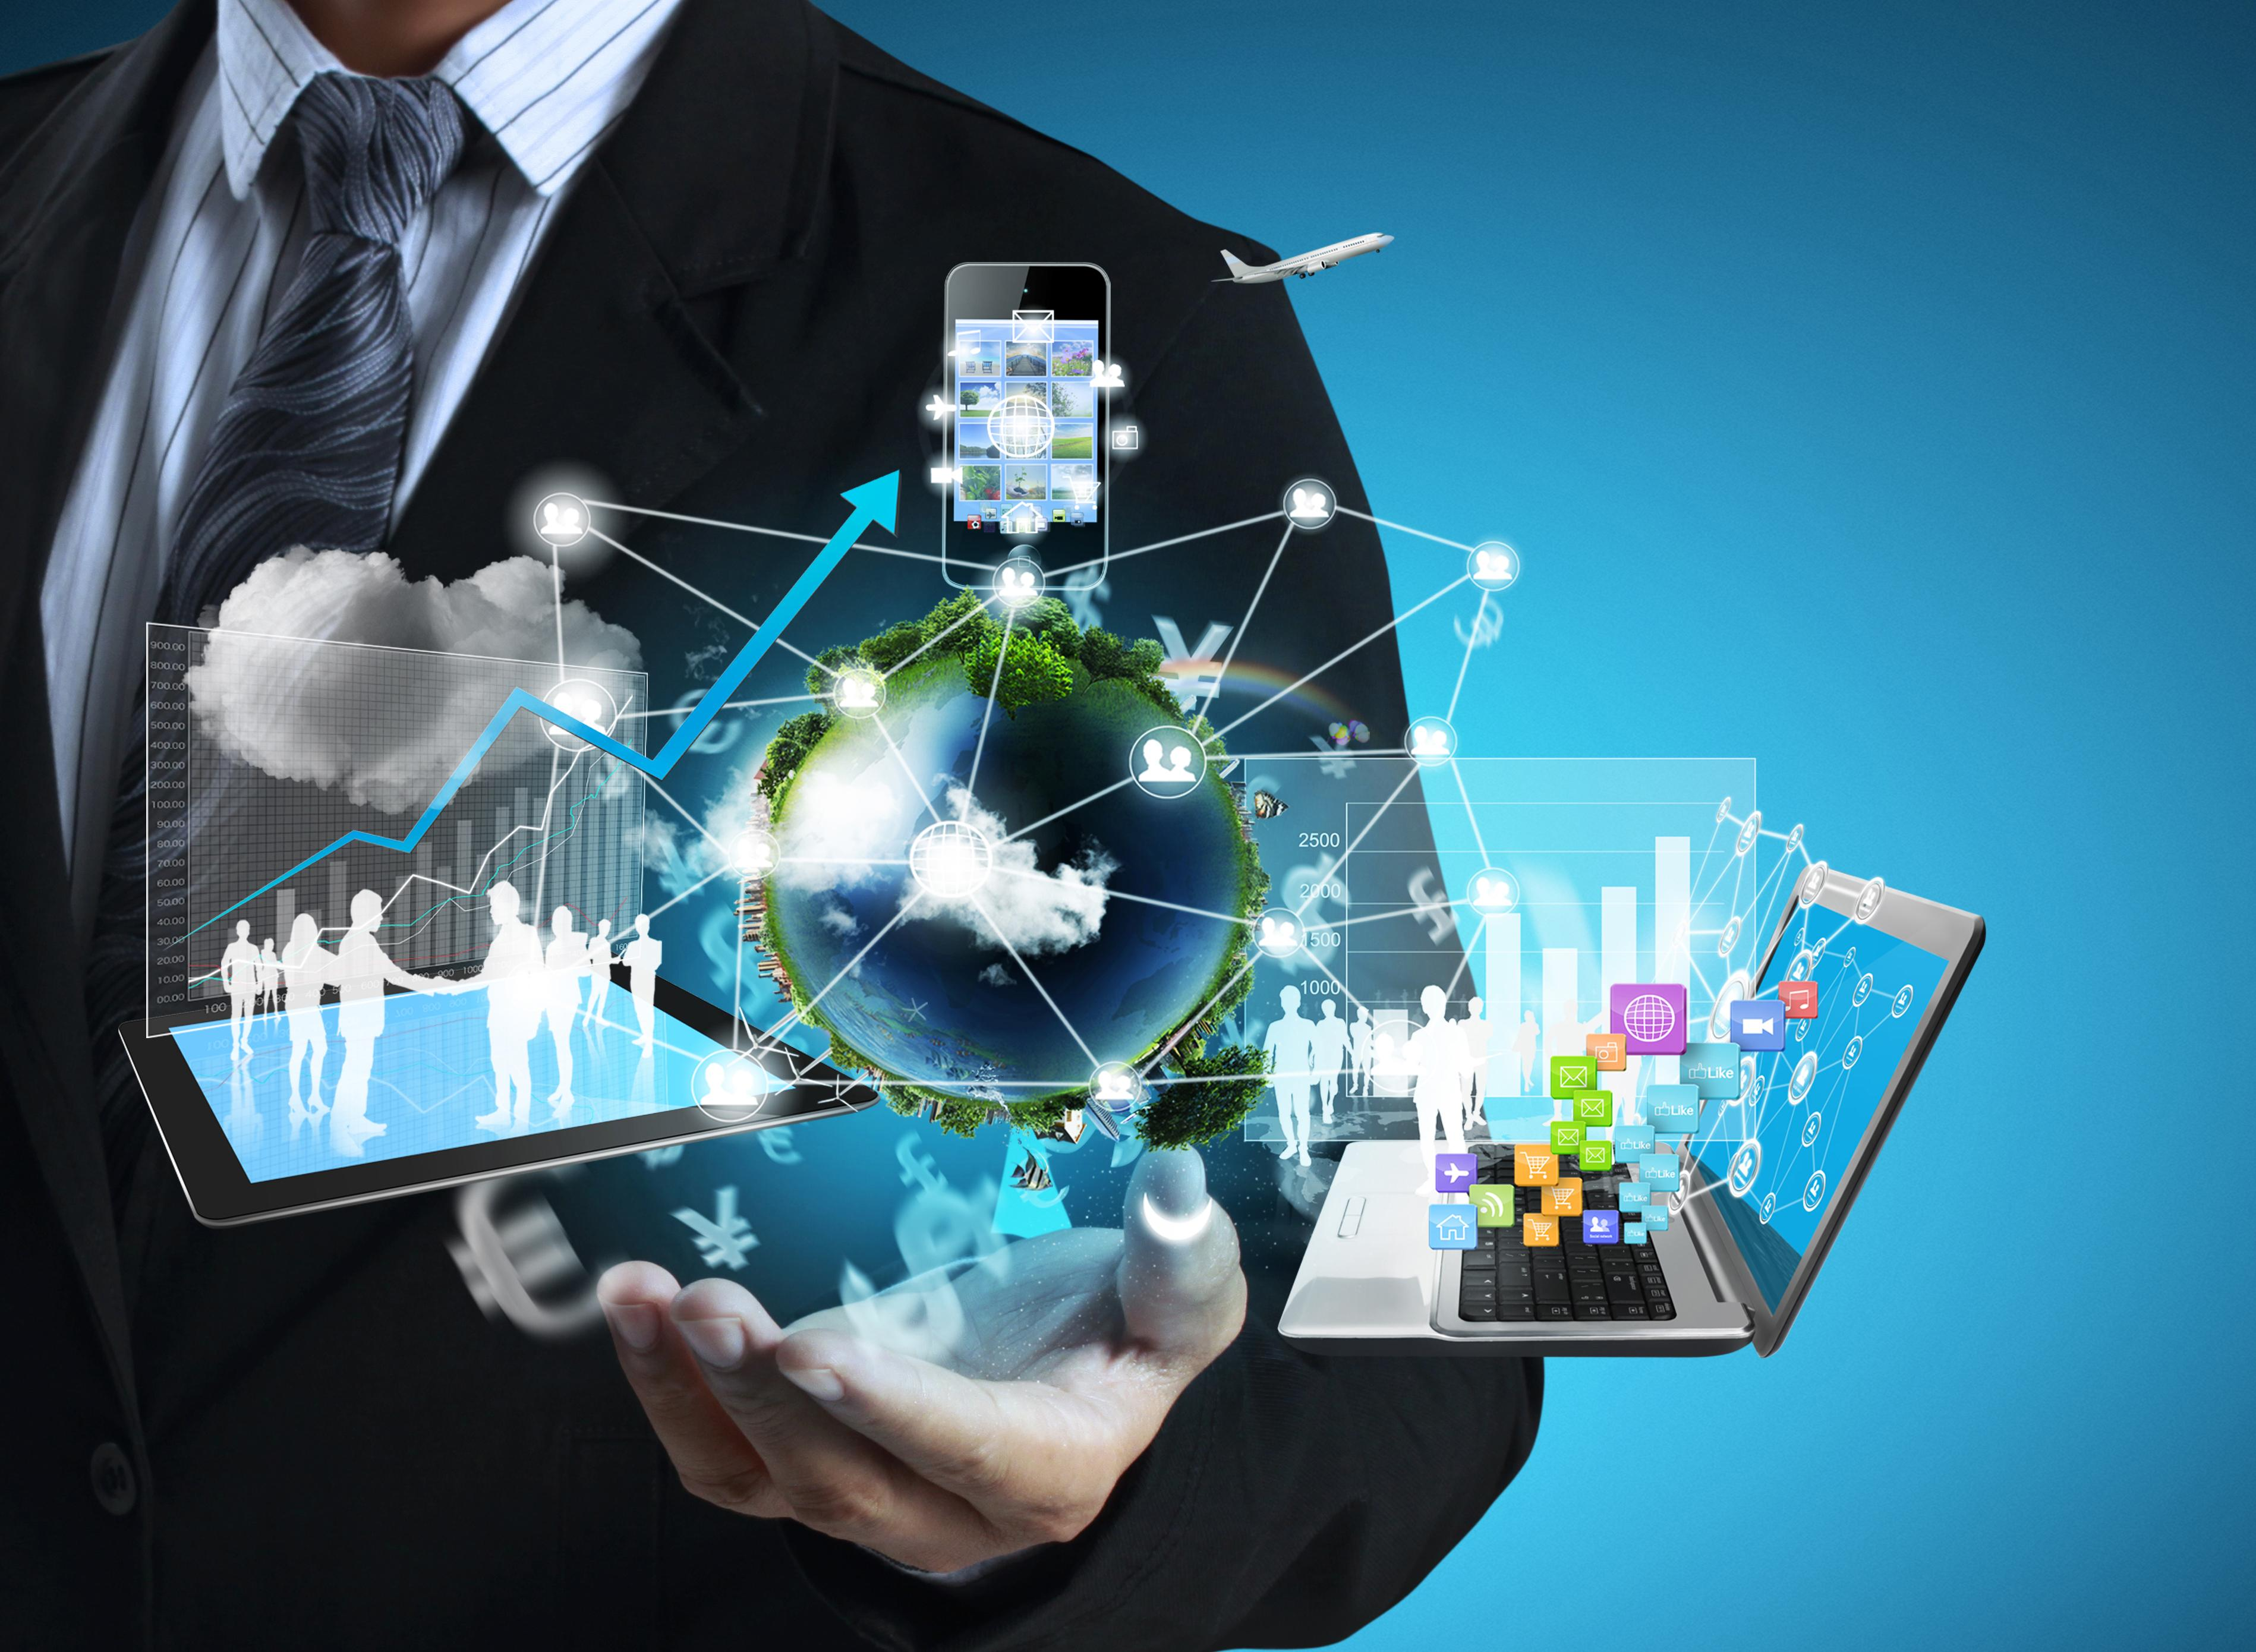
\includegraphics[width=\textwidth]{figures/tech.jpg}
	\end{frame}

	\begin{frame}{How is Location Privacy \& Security Understood?}
		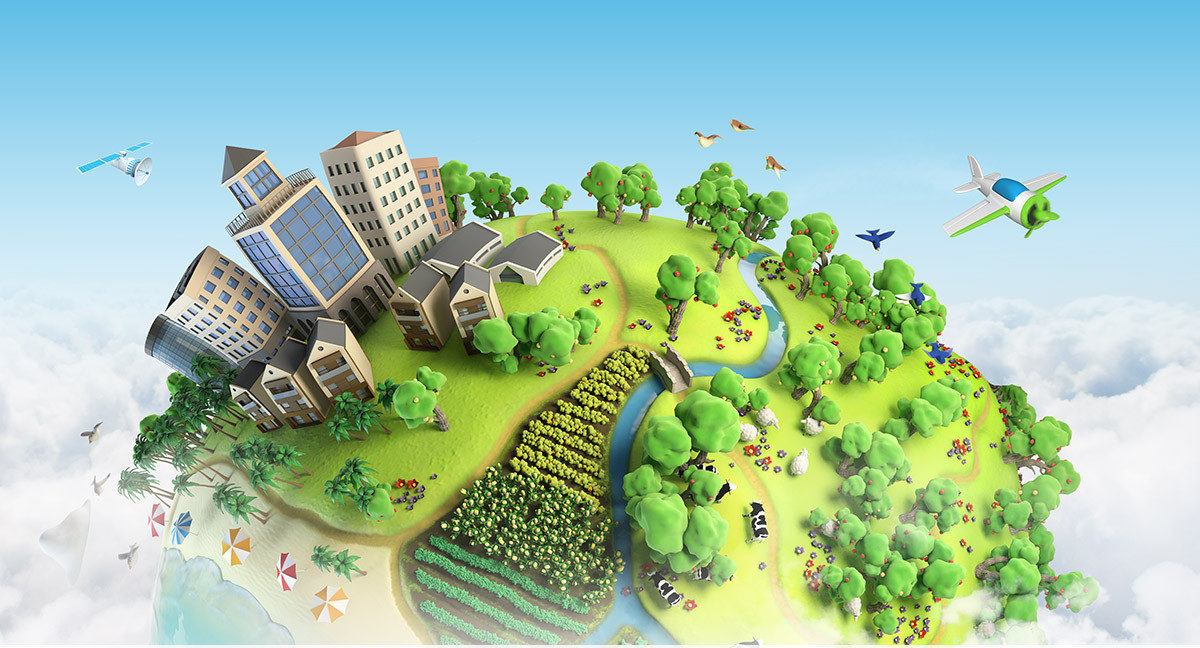
\includegraphics[width=\textwidth]{figures/gis.jpg}
	\end{frame}

	\begin{frame}{Media}
		\begin{figure}
			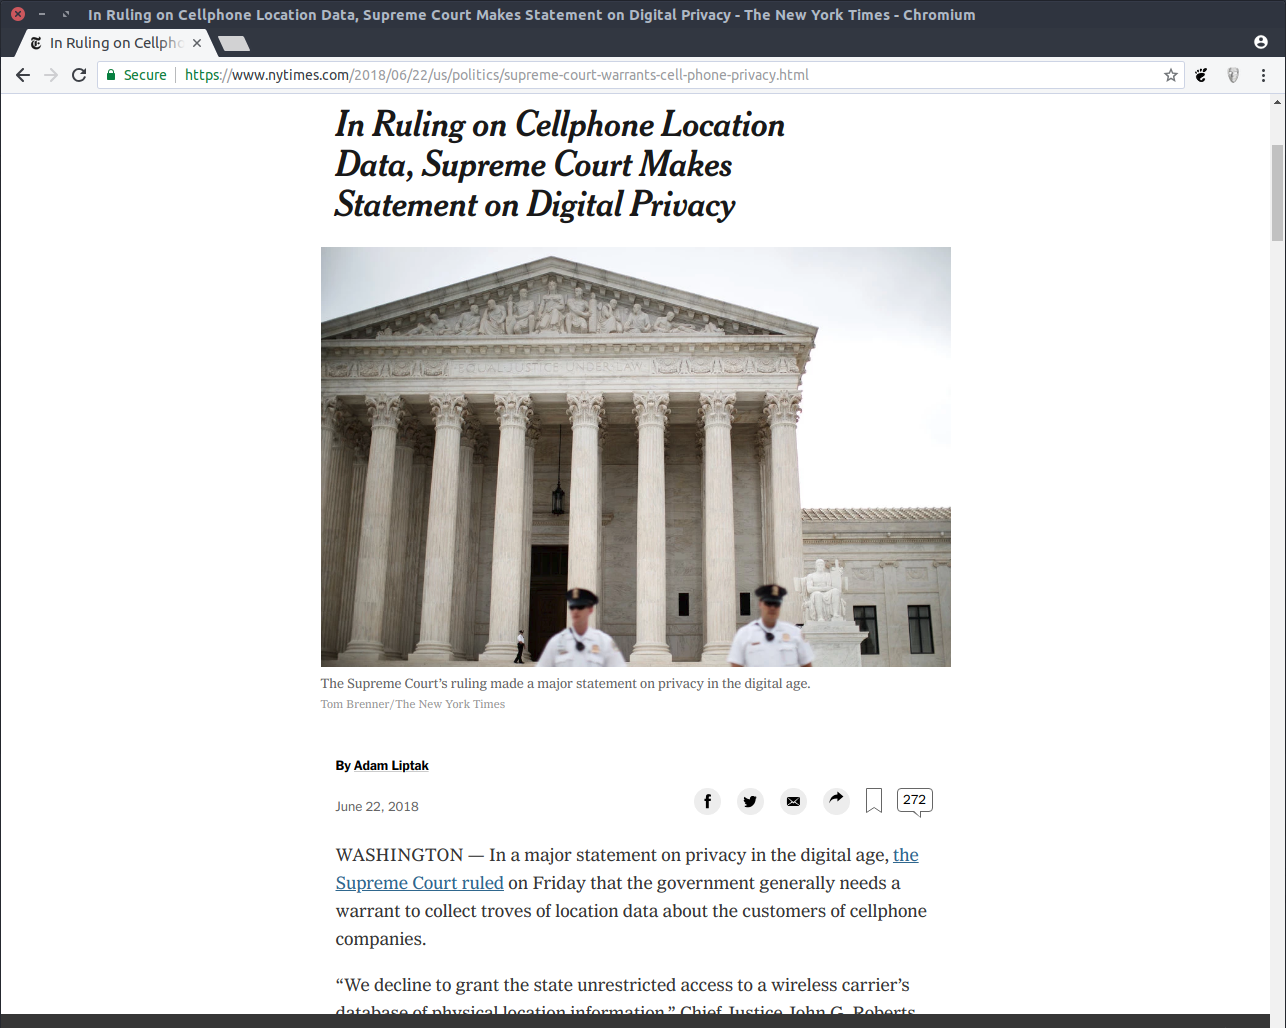
\includegraphics[width=0.49\textwidth]{figures/news1.png}
			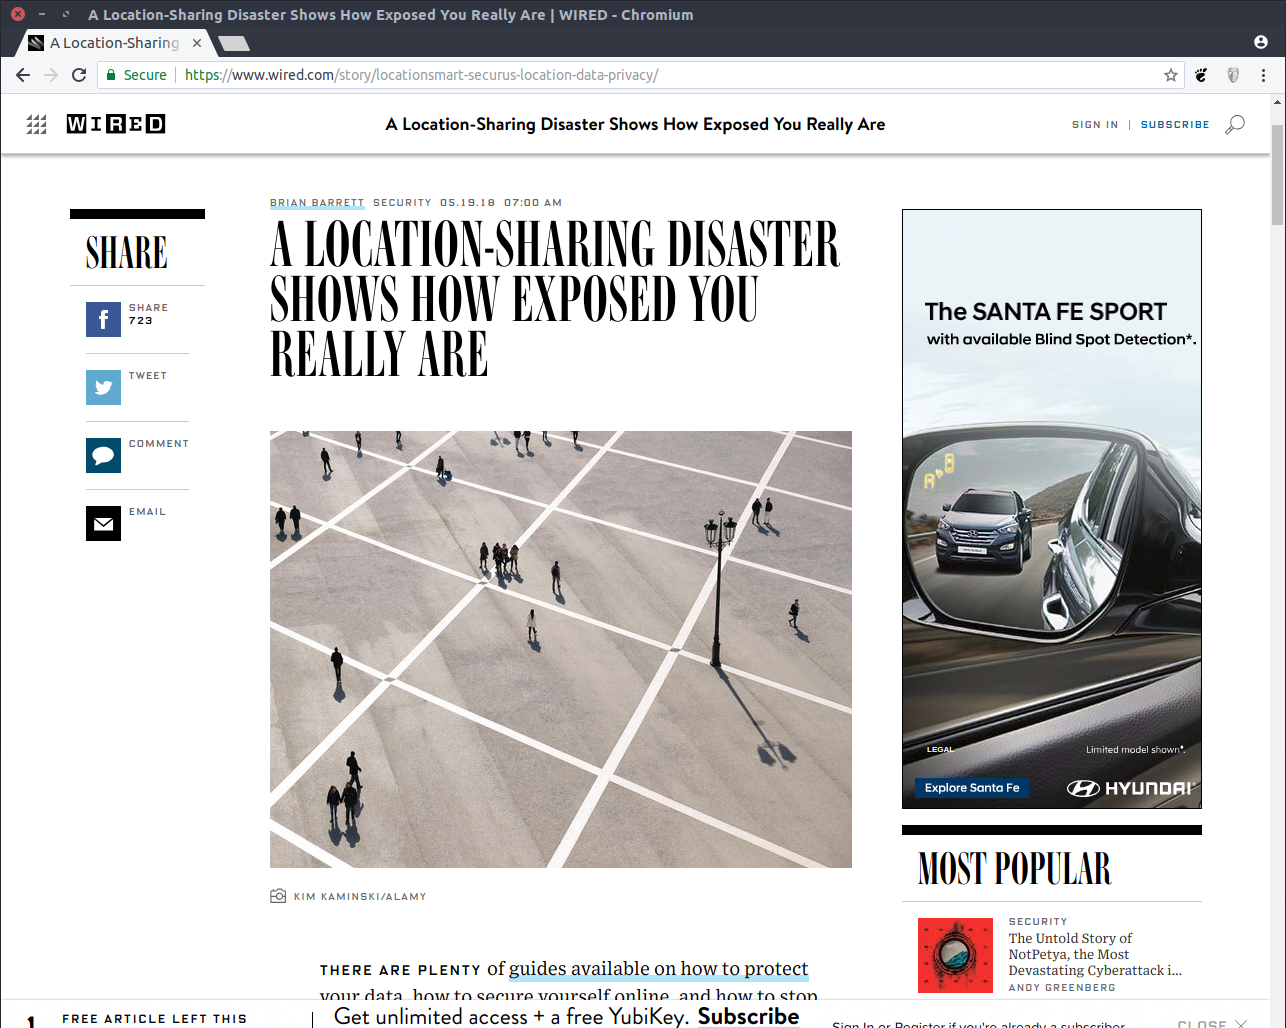
\includegraphics[width=0.49\textwidth]{figures/news2.png}
			
			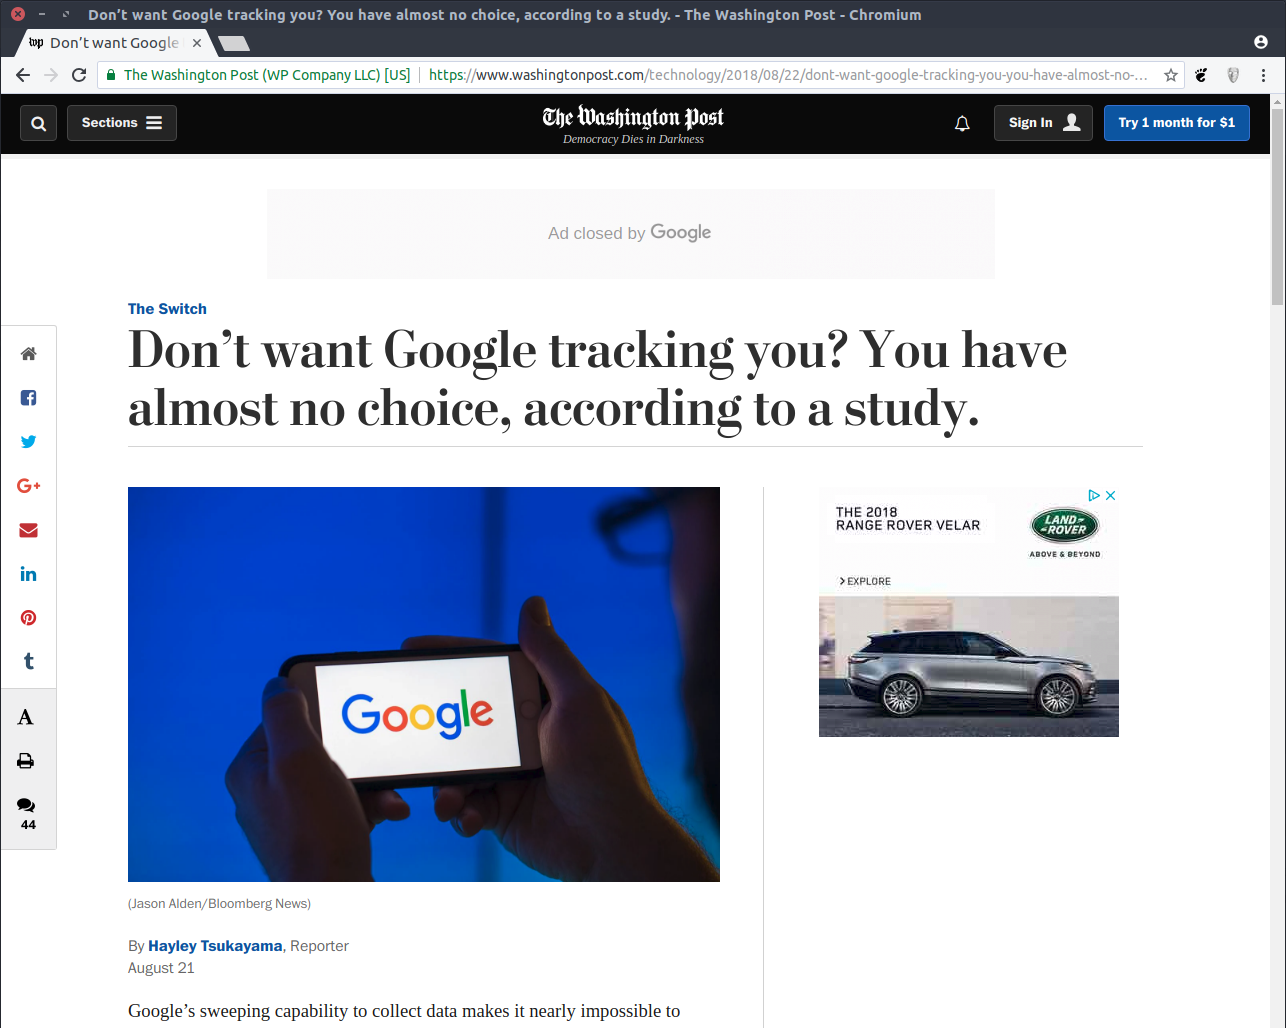
\includegraphics[width=0.49\textwidth]{figures/news3.png}
			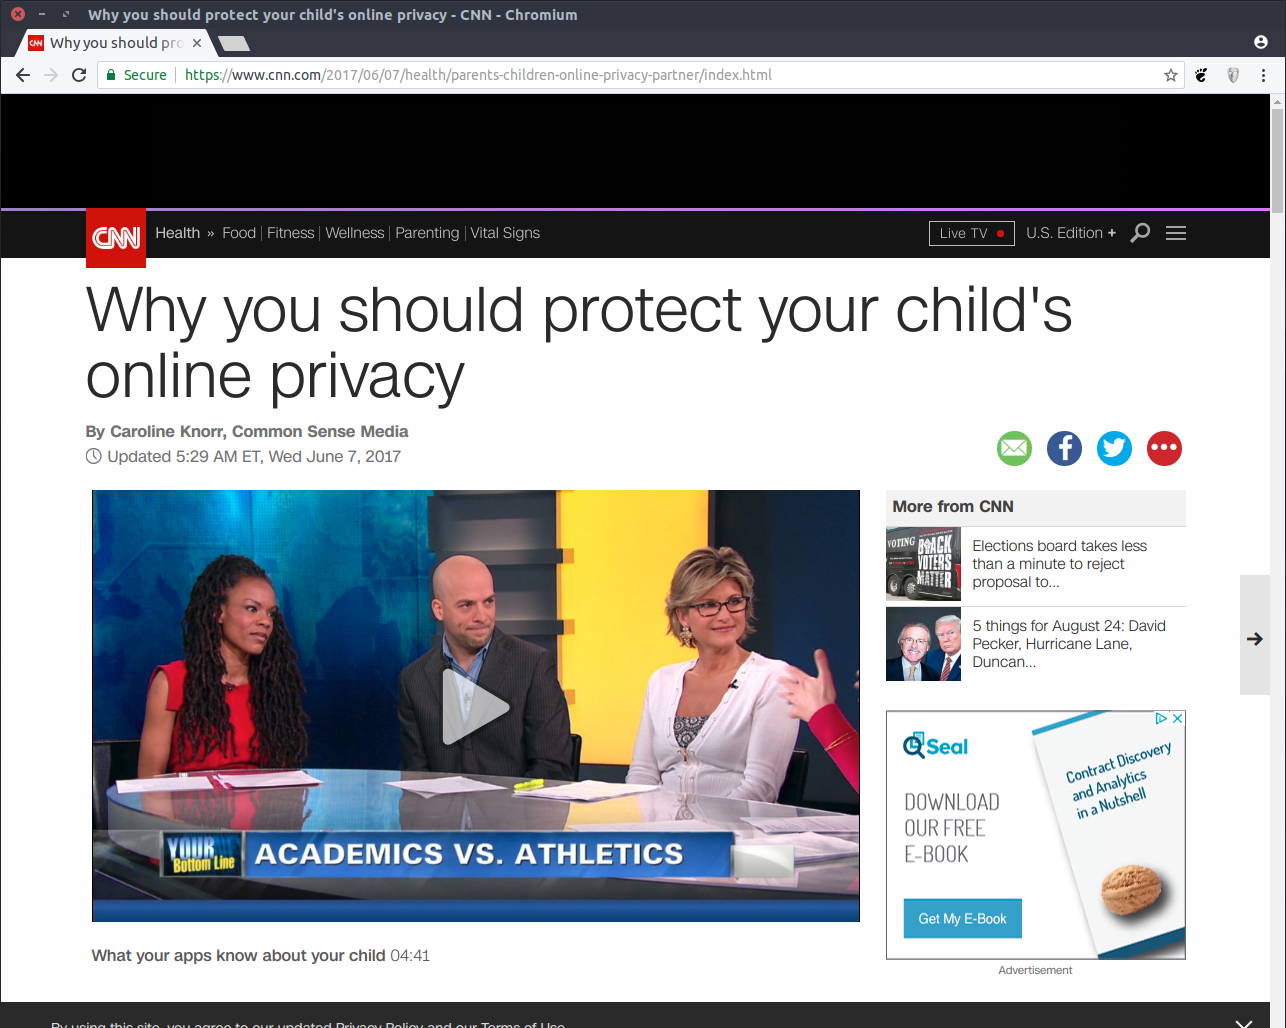
\includegraphics[width=0.49\textwidth]{figures/news4.png}
		\end{figure}
	\end{frame}

	\begin{frame}{LoPaS '18}
		\begin{itemize}
			\setlength\itemsep{1em}
			\item Purpose of this workshop is to bring together researchers interested in Location Privacy \& Security.
			\pause
			\item Computational methods and technology are an important topic, but so are the social, ethical, institutional, legal, etc. components.
			\pause
			\item This workshop is intended to be a true \texttt{workshop} rather than another mini-conference.
			\pause
			\item Lots of time for discussion, collaborating, setting targets/goals.
		\end{itemize}
	\end{frame}

	\section{Who}

	\begin{frame}{LoPaS '18}
		\textbf{Organizers}
		\begin{itemize}
			\item Grant McKenzie
			\item Carsten Ke{\ss}ler
			\item Clio Andris
		\end{itemize}
		\textbf{Program Committee}
		\begin{itemize}
			\item Marc P. Armstrong, University of Iowa
			\item Carson Farmer, University of Colorado, Boulder
			\item Sebastien Gambs, Université du Québec à Montréal
			\item Yingjie Hu, University of Tennessee, Knoxville
			\item Krzysztof Janowicz, University of California, Santa Barbara
			\item Peter Johnson, University of Waterloo
			\item Bernd Resch, University of Salzburg
			\item Colin Robertson, Wilfrid Laurier University
			\item Dara Seidl, San Diego State University
			\item Martin Tomko, University of Melbourne
		\end{itemize}
	\end{frame}

	\begin{frame}{LoPaS '18}
		\textbf{Accepted Papers}
		\begin{itemize}
			\setlength\itemsep{1em}
			\item Seeking Mr \& Ms Regular: Sentinels to Characterize Crowd Dynamics\\
			\texttt{Elham Naghizade, Jeffrey Chan, and Martin Tomko}
			\item Exploring the Effectiveness of Geomasking Techniques for Protecting the Geoprivacy of Twitter Users\\
			\texttt{Song Gao and Qunying Huang}
			\item trajGANs: Using generative adversarial networks for geo-privacy protection of trajectory data\\
			\texttt{Xi Liu, Hanzhou Chen, and Clio Andris}
			
		\end{itemize}
	\end{frame}

	\begin{frame}{Program}
		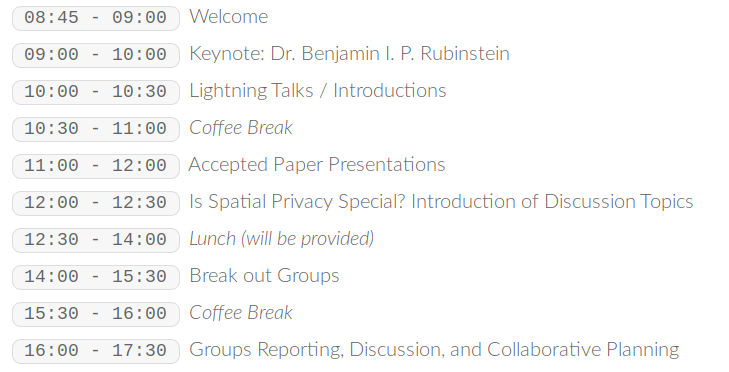
\includegraphics[width=\textwidth]{figures/program.png}
	\end{frame}

	\begin{frame}{JoSIS Special Issue}
		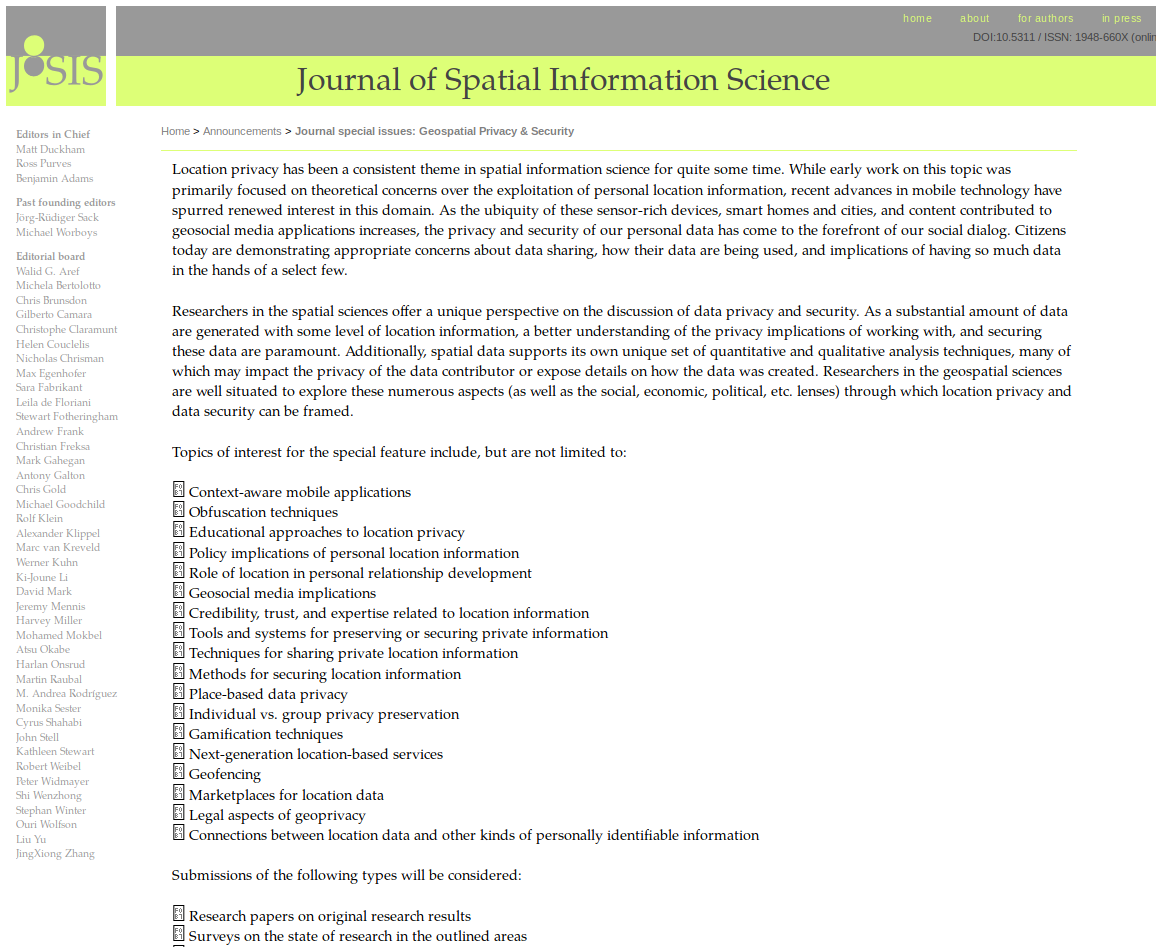
\includegraphics[width=\textwidth]{figures/specialissue.png}
	\end{frame}

	\begin{frame}{Keynote}
	
		\Large \textbf{Towards Turn-Key Differential Privacy}
		
		\vspace{5mm}
		
		\normalsize
		
		\textbf{Dr. Benjamin I. P. Rubinstein}\\
		\texttt{\footnotesize{Associate Professor\\School of Computing \& Information Systems\\University of Melbourne}}\\
		
		
		
		
	\end{frame}

\usebackgroundtemplate%
{%
	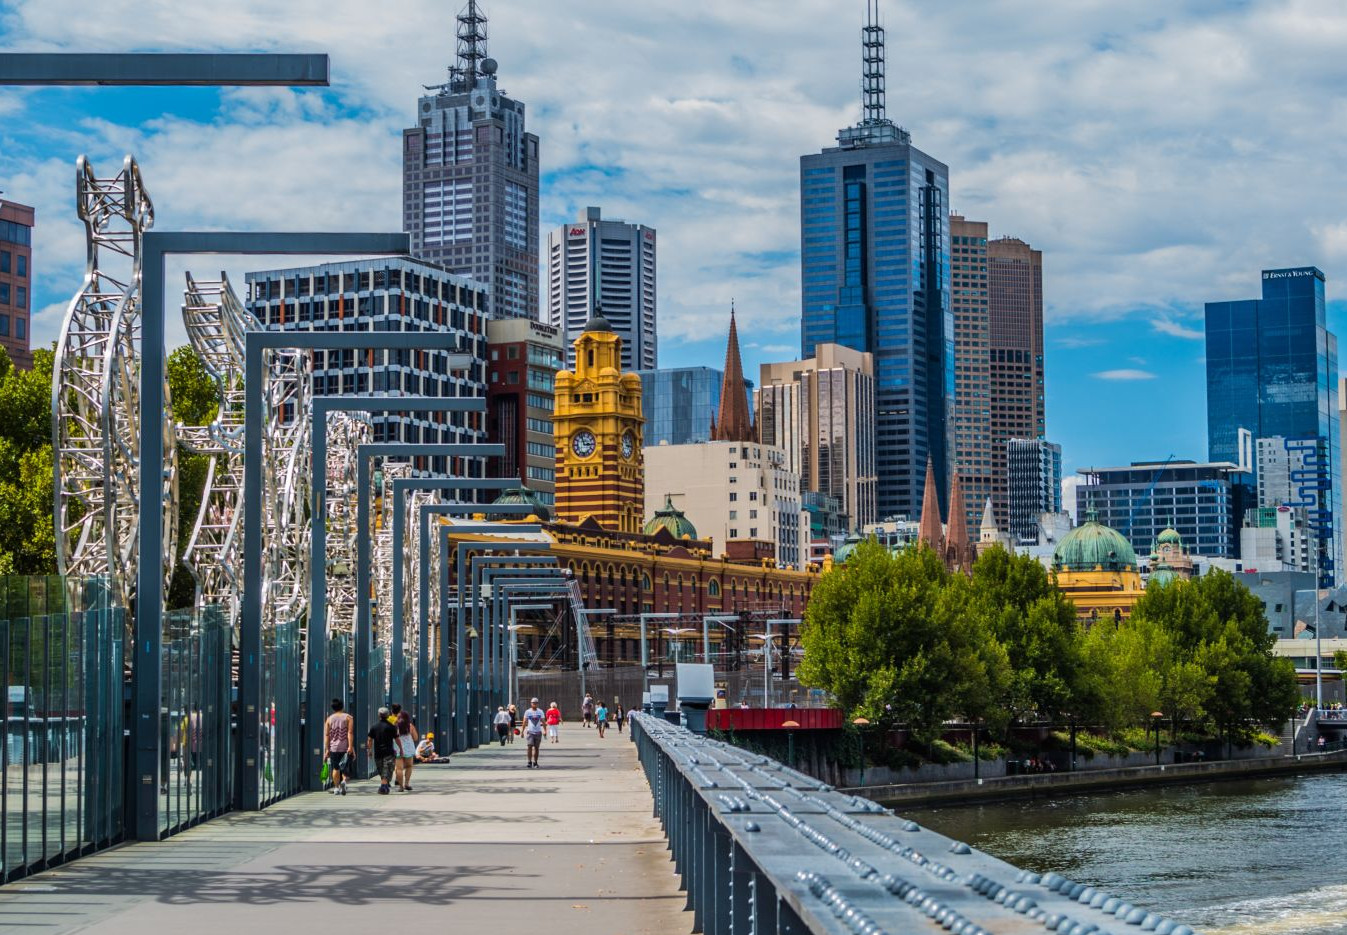
\includegraphics[width=\paperwidth,height=\paperheight]{figures/melbourne.jpg}%
}

	\begin{frame}

		\begin{tikzpicture}[overlay]
		\draw [transform canvas={yshift=-7.7cm,xshift=-1.1cm}, draw=white, fill=white, opacity=0.8] (0,0) rectangle (13.1,5.9);
		\end{tikzpicture}
		\titlepage
	\end{frame}
	
\end{document}


